\section{WebshopSimulator} \label{prog}

Webapplikasjonen som DBUpgradinator testes på, kalles for \emph{WebshopSimulator}. Dens arkitektur følger både det logiske, det prosessmessige og det fysiske perspektivet skissert i figurer \ref{fig5}, \ref{fig6}, \ref{fig7}, \ref{fig8}, \ref{fig9}, og \ref{fig10}. Testapplikasjonen etterkommer også systembegrensningene opplistet i delkapittel 4.2.2. Dette delkapitlet skisserer strukturen til testapplikasjonens kildekode, dets avhengigheter, og hvordan tjenerprogrammet blir kompilert til en kjørbar .jar - fil.

\subsection{Simulasjon av brukerforespørsler}

Et klientprogram, skrevet i Javscript, genererer og sender forespørsler til det simulerte produksjonsmiljøet DBUpgradinator testes i. Dette skriptet kjøres i kjøretidsmiljøet NodeJS, fra en norsk datamaskin i Trondheim. Klientprogrammet kalles for \emph{WebAppSimulator}\footnote{Kildekoden til simulatoren er tilgjengelig fra URL \url{https://github.com/vegardbb/DBUpgradinator/tree/master/demo/webappsimulator}.}. Dets hovedoppgave er å simulere en kontinuerlig serie med forespørsler som jevnfordeles blant applikasjonsinstansene. Programmets funksjonalitet kan i korte trekk inndeles i tre satser:

\begin{enumerate}
  \item Programmet sender klyngen av tjenere en serie av POST-forespørsler, slik at nye aggregater lagres på hver av de tomme nodene i databasen. Den totale datamengden som sendes over TCP/IP er begrenset til under én gigabyte, slik at testingen ikke tar altfor lang tid. Samtidig holder en egen loggeprosess styr på ID-verdiene som genereres av tjenerne som tilsendes denne simulerte klienten
  \item Etter at den første satsen er ferdig, terminerer programmet. Da må applikasjonsloggene til hver av tjenerinstansene transformeres til én liste av unike IDer. Til å oppnå dette formålet brukes tekstbehandlingsverktøyet Vim, en kommandolinjeapplikasjon som kan redigere alle linjer i loggen samtidig ved hjelp av regulære uttrykk og dets kraftige kommandolinjesyntaks. Dernest må klientsimulasjonsprogrammet redigeres slik at listen av aggregat-IDer blir lest inn fra korrekt filsti, og slik at funksjonen som kjører den tredje satsen blir kjørt neste gang programmet blir startet opp fra kommandolinjen
  \item Programmet sender applikasjonstjenerne én HTTP-forespørsel per ID i listen som ble oppretttet i forrige steg. Hver forespørsel kan enten være en PUT \- forespørsel eller en GET \- forespørsel. Funksjonen \texttt{Math.random()} brukes til å bestemme hvilket av de to verbene forespørselen kaller på en tjener
\end{enumerate}

For å generere data til POST - forespørslene i steg 1 og PUT - forespørslene i steg 3, brukes en komma\-separert seed-fil som inneholder en tabell der hver rad har en strengverdi for fornavn, etternavn, telefonnummer, gateadresse, poststed, delstat, postkode, og land\footnote{Navn - og addresser i seed-filen stammer fra gratistjenesten Fake Name Generator, som tilbyr inntil 100 000 navn og addresser i en kommaseparert fil per bestilling. URL: \url{https://www.fakenamegenerator.com/order.php}}. Simulasjonsprogrammet leser inn seedfilen og grupperer hver av kolonnene i tabellen til et sett med lister, der hver liste er assosiert med ett av de åtte tidligere nevnte kolonnenavnene.

Ved hjelp av pakken ''node-fetch'' genererer skriptet HTTP-forespørsler asynkront, det vil si at det ikke venter på svar fra applikasjonstjenerne for hver tilsendt forespørsel før den neste sendes. En funksjon i skriptet, kalt \texttt{chooseRandom}, returnerer et pseudotilfeldig valgt element fra et liste-parameter. Denne funksjonen brukes til å velge en tilfeldig applikasjonstjener som skal motta en forespørsel, fra en liste av URL-er. Den samme funksjonen kalles på for å generere hvert attributt i et aggregat som enten skal postes eller oppdateres i databasen. Prosedyren for generering av PUT - forespørsler skiller seg ut fra generering av POST-forespørsler og med at PUT-endepunktet til WebShopSimulator sitt ReST-API krever et \emph{id}-parameter.

Skriptet bruker et separat loggeobjekt, som instansieres ved hjelp av pakken Winston\footnote{Publisert på npm. URL: \url{https://www.npmjs.com/package/winston}}. Loggeobjektet logger responsen applikasjonstjenerne sender tilbake for hver genererte forespørsel.

\subsection{Programvare på tjenerne}

% Om webapplikasjonen, dets kildekode, avhengigheter og bygging
Kildekoden til WebShopSimulator er åpent tilgjengelig på DBUpgradinator sitt GitHub - repositorium: \url{https://github.com/vegardbb/DBUpgradinator/tree/master/demo/WebshopSimulator}. Programmet er et Java - prosjekt som bruker DBUpgradinator til å oppgradere sin datamodell. Programmet er en webapplikasjon som eksponerer et ReST-API til mange nettleserklienter. Klassediagrammet i figur \ref{classfig} viser den statiske relasjonen mellom kildekoden til DBUpgradinator og kildekoden til WebShopSimulator.

% Figur 11
\begin{figure}[hbtp]
  \centering
  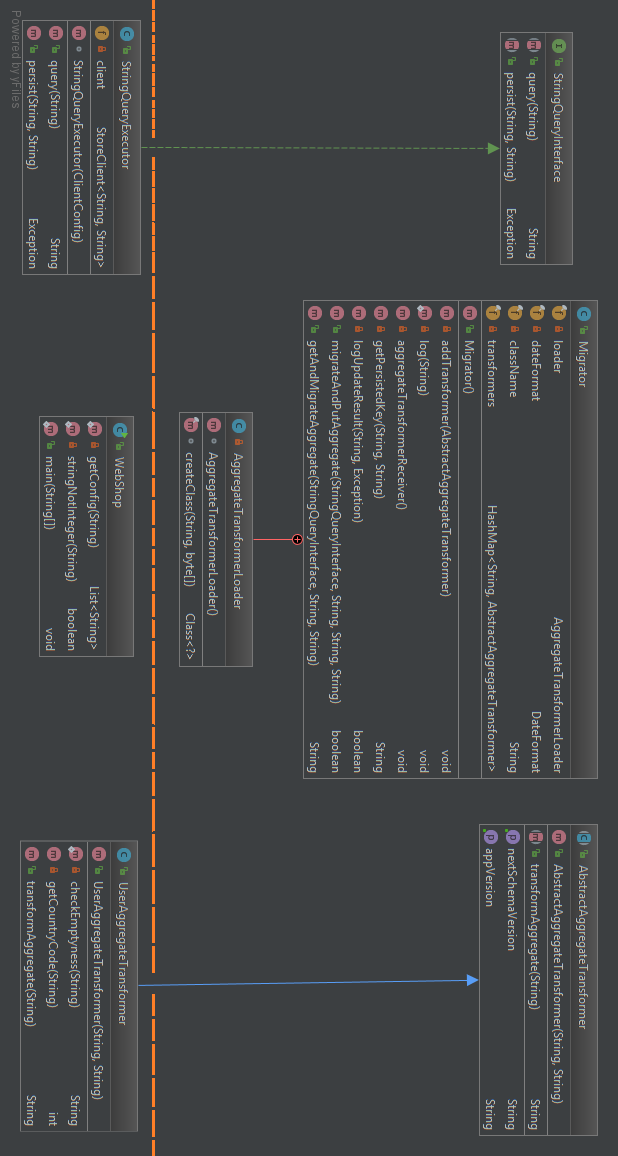
\includegraphics[scale=0.59]{fig/class-diagram.png}
  \caption{Klassediagram av WebShopSimulator. Den gule, stiplete linjen markerer et skille mellom klassene til DBUpgradinator og klassene til WebShopSimulator.}
  \label{classfig}
\end{figure}

For å realisere ReST-APIet til den typiske webapplikasjon DBUpgradinator er ment å operere på (se også figur \ref{fig5}), ble Java-pakken Spark\footnote{Må ikke forveksles med Apache Spark, som er et distribuert dataprosesseringsverktøy ment for stordata-systemer.} benyttet. Spark er et mikro\-rammeverk laget for at utviklere kan skrive en webapplikasjon sentrert rundt mikrotjeneste\-mønsteret lettere og raskere. Applikasjonen har i hovedsak tre ruter i sitt grensesnitt:

\begin{description}
  \item[GET /api/:id?schema=x] Applikasjonen leser det aggregatet i databasen som har nøkkelprefiks lik \emph{:id} og skjemasuffiks lik \emph{x}
  \item[PUT /api/:id?schema=x] Applikasjonen oppdaterer det aggregatet i databasen som har nøkkelprefiks lik \emph{:id} og skjemasuffiks lik \emph{x}
  \item[POST /api?schema=x] Applikasjonen oppretter et nytt aggregat (ut i fra forespørselens ''body'' - variabel) i databasen som tilhører skjemaversjon \emph{x}
\end{description}

I kildekoden til WebShopSimulator er det også skrevet en separat klasse, som utifra en instans av VoldemortClientConfig instansierer et StoreClient - objekt. Dette objektet koordinerer og utfører spørringer over TCP - forbindelser med hver av databasenodene i Voldemort-instansen som kjører i testmiljøet. Selve klassen i WebShopSimulator implementerer grensesnittet \texttt{StringQueryInterface}, som er listet opp i kodeoppføring \ref{queryinter}.

Artefaktene benevnt i \ref{fig10} som ''DBUpgradinator.jar'' og ''WebShopSim.jar'' ble bygget i utviklingsmiljøet IntelliJ IDEA. I dette programmet kan man definere underprosjekter, eller ''moduler'', innen et Java-prosjekt. Enhver modul har sin egen katalog for å ha kildekode i. Avhengigheter, det vil si artifakter som inneholder klasser som importeres inn i kildekoden, registreres i en modul. Før en \texttt{.jar} - fil kan kompileres og bygges må en artefakt defineres. IntelliJ knytter hver artifakt til en modul. Slik kan Intellij legge ved de \texttt{.jar} - filene artifakten trenger for å kunne fungere ordentlig.

DBUpgradinator er utstyrt med en enkel, hjemmelaget loggefunksjon. Denne loggeren påkalles hver gang et aggregat har blitt migrert til et nytt skjema, og hver gang et aggregat er blitt bekreftet skrevet til disk av databasenodene. Loggfunksjonen skriver et klokkeslett på formen \texttt{åååå-mm-dd hh:mm:ss}. Ved hjelp av loggingen kan man teste hvordan den levende datamigrasjonen påvirker en applikasjons evne til å betjene forespørsler til dens klienter.

\subsection{Konfigurasjon av Voldemort-instans}

Databaseklyngens modus operandi reguleres av tre forskjellige konfigurasjonsfiler:

\lstinputlisting[style=xml, label=cluster, caption={cluster.xml - filen definerer de fire nodene i databaseklyngen til testmiljøet.}]{code/conf/cluster.xml}

Klyngekonfigurasjonen holder på variabler som er konsistent like for samtlige noder (det være seg kjørende database\-tjener\-prosesser) i Voldemort-instansen. Eksempler på slik informasjon inkluderer nodenes vertsnavn, id, og tilkoplingsport for TCP-forbindelser med \textbf{StoreClient} - instanser \citep{kreps2009}. I \texttt{cluster}-konfigurasjonen defineres også alle partisjonene som er spredd utover nodene.

Fordelingen av disse partisjonene påvirker fordelingen av nøkler i den konsistente hashringen. Mens en Voldemort-instans er oppe kan disse partisjonene omfordeles fritt, men de kan i sum aldri bli færre eller flere. De øvrige konfigurasjonsvariablene må være konstante gjennom hele databaseinstansens livsløp, og de må være like for alle nodene i klyngen \citep{kreps2009}.

Hvis produksjonsmiljøet opererer med flere databasetjenere på samme datasenter, og samtidig kjøres på tvers av flere datasentre, går det an å definere soner innenfor klyngen. Dens funksjonelle verdi er å unngå at to replikaer for samme nøkkel havner på samme datasenter. I tilfellet med testmiljøet til WebShop hadde det vært hensiktsmessig å inndele klyngen i to soner: Nodene som er lokalisert i Frankfurt og nodene som er lokalisert utenfor Frankfurt. Dette er imidlertid ikke gjort for databaseklyngen WebShopSimulator opererer på.

\lstinputlisting[language=python, label=serverproperties, caption={\texttt{server.properties} er filen som bestemmer oppførselen til den enkelte databasenode i databaseklyngen.}]{code/conf/server.properties}

En minimal tjenerkonfigurasjon inneholder én linje, og det er den som definerer id-en til noden. Dette er påkrevd, slik at noden vet hvilken nodekonfigurasjon fra \texttt{cluster.xml} det er som skal leses. Som vist i kodeoppføring \ref{serverproperties}, definerer tjener\-konfigurasjons\-filen kjøretidsegenskapene til persisterings\-motoren BDB Java, som alle de fire nodene tar ibruk for å lagre data.

\lstinputlisting[style=xml, label=test, caption={En STORE - fil som bestemmer hvordan data lagres i databasen.}]{code/conf/test.xml}

Quorum-konfigurasjonen bestemmes ikke i \texttt{cluster.xml}, da det noen ganger kan være ønskelig at noen aggregater skal kunne gjøres mer tilgjengelige enn andre. Quroum-parameterne \(R\), \(W\), og \(N\) defineres for hvert nøkkelverdi\-lager i klyngen, altså defineres de i filen \texttt{test}, henholdsvis med nøkkelordene \emph{required-reads}, \emph{required-writes}, og \emph{replication-factor}. I konfigurasjonen beskrivet av oppføring \ref{test} kan man se at databasen fører en ''strict quorum'' - policy, jamfør kapittel \ref{strictquorum}.

\texttt{test} - filen er konfigurasjonsfilen til nøkkelverdi-lageret hvis identifiserte navn er ''test''.  I prinsippet kan en databaseklynge ha flere databaseinstanser, men det går ikke an å kjøre spørringer på tvers av dem. Filen dikterer hvilken strategi nodene skal følge når de leverer antydede replika\-aggregat til sine midlertidige addresser.

Kodeoppføring \ref{test} definerer også serialiseringsmetoden nodene benytter når de lagrer aggregater mottat fra en spørringskoordinator. I dette tilfelle heter denne metoden ''string'', det vil si at oktettene noder mottar behandles som UTF8-kodet tekst.

\subsection{Testmiljø}

% Kap. 5.2.4
Deployment-diagrammet fra figur \ref{fig10} beskriver testmiljøet DBUpgradinator skal testes i. De fire boksene refererer til fire forskjellige datasentre. Hver enkelt av de fire applikasjonsnodene gjestes av skyinfrastrukturleverandøren DigitalOcean, og alle er spredd utover tre forskjellige datasentre i London (LON1), Amsterdam (AMS3), og Frankfurt am Main (FRA1). I hvert datasenter betjenes én virtuell maskin, eller \underline{droplet}, som DigitalOcean kaller dem.

Hver av de virtuelle maskinene modellert i figur \ref{fig10} kjører samme operativsystem, versjon 8.10 av Debian GNU/Linux. Alle har hver én gigabyte med arbeidsminne. Hver av maskinene disponerer et eget SSD-lager med en kapasitet på 25 GB, og én sepaprat, virtuell prosesseringsenhet.

% Tabell som viser statistikk for HTTP-forepsørslene sendt i test 3
\begin{table}[!h]
\begin{center}
    \begin{tabular}{ | l | l | l |}
      \hline
      \textbf{Vertsnavn} & \textbf{IP-adresse} & \textbf{Datasenter} \\ \hline
      vbb-master2018-avery & 167.99.84.243 & LON1 \\ \hline
      vbb-master2018-black & 188.166.103.205 & AMS3 \\ \hline
      vbb-master2018-crabbe & 206.81.31.127 & FRA1 \\ \hline
      vbb-master2018-dolohov & 206.81.31.128 & FRA1 \\ \hline
    \end{tabular}
\end{center}
\caption{Oversikt over virtuelle datamaskiner brukt under testing av DBUpgradinator.}
\label{droplets}
\end{table}


I tabell \ref{droplets} oppgis vertsnavnene og IPv4 - addressene til hver av de virtuelle maskinene, samt hvilket datasenter hver av de er opprettet i. Assosiasjonen mellom navnet til vertsmaskinene og datasentra er også gjengitt i figur \ref{fig10}.

